\documentclass{article}
\usepackage[margin=2.5cm]{geometry}
\usepackage{amsmath,amssymb}
\usepackage{graphicx}
\usepackage{tikz}
\usetikzlibrary{arrows.meta,positioning}

\begin{document}

\chapter{Implementation}\label{chap:implementation}

This chapter describes the implementation of the proposed smart walker system that integrates a vision--language model (VLM) based on Qwen2.5-VL into the perception and shared-control pipeline. The goal is to explain the architecture in sufficient detail for a technically literate reader, while keeping the mathematics and design choices accessible.

\begin{figure}[t]
        \centering
        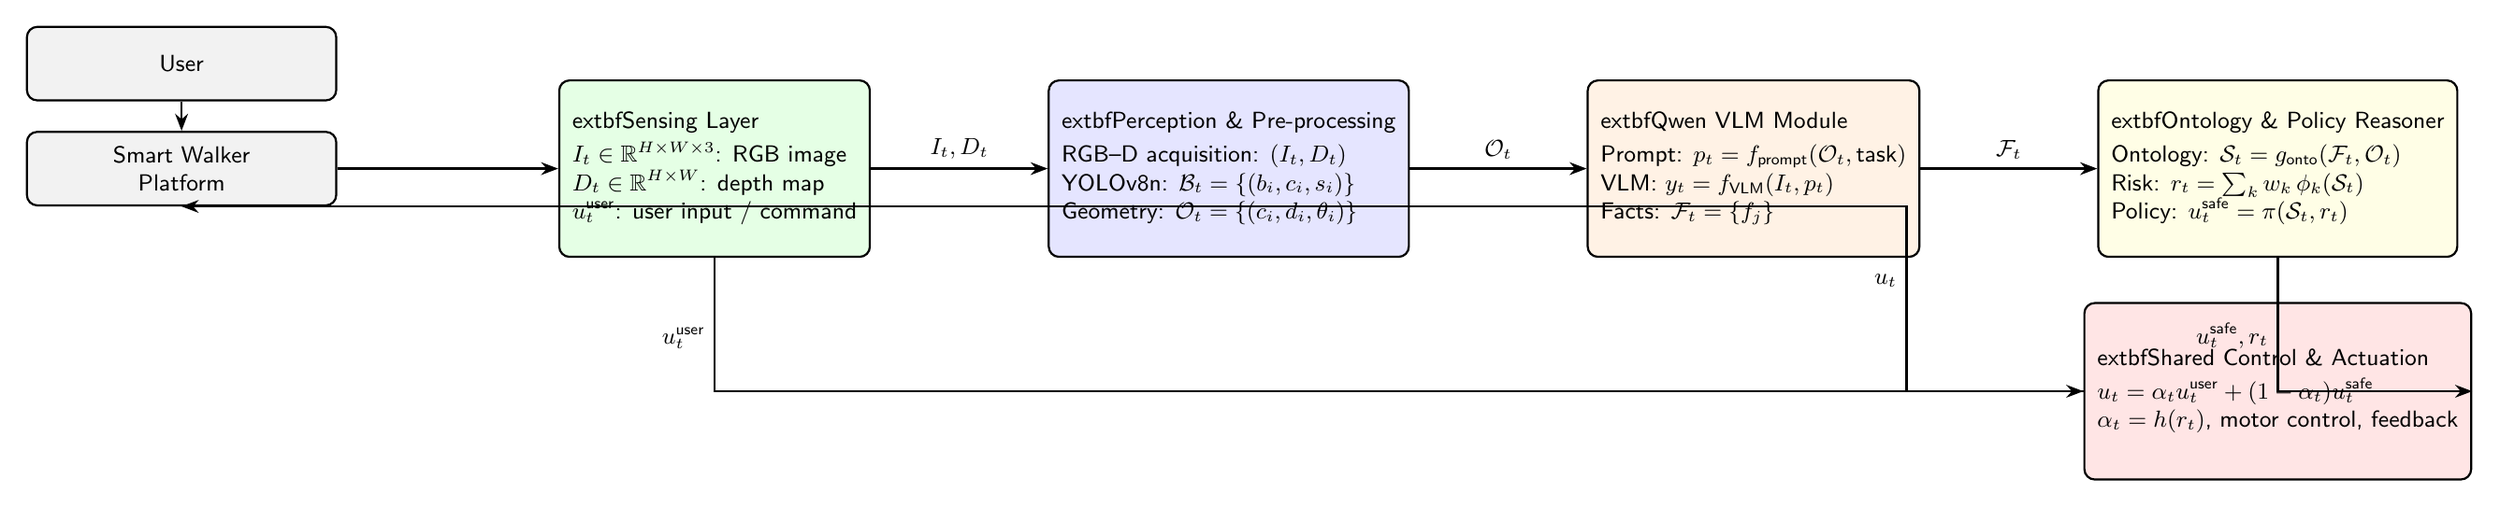
\begin{tikzpicture}[
            font=\sffamily\small,
            layer/.style={rectangle, rounded corners, draw=black, thick,
                                        minimum width=4.2cm, minimum height=2.4cm,
                                        align=left, inner sep=5pt},
            flow/.style={->, >=Stealth, thick},
            every node/.style={align=center}
        ]

        % User and platform
        \node[layer, fill=gray!10, minimum height=1.0cm, align=center] (user)
            {User};
        \node[layer, fill=gray!10, minimum height=1.0cm, align=center,
                    below=0.4cm of user] (platform)
            {Smart Walker\\Platform};

        % Sensing layer
        \node[layer, fill=green!10, right=3.0cm of platform, anchor=west] (sensing) {%
            	extbf{Sensing Layer}\\[2pt]
            $I_t \in \mathbb{R}^{H\times W\times 3}$: RGB image\\
            $D_t \in \mathbb{R}^{H\times W}$: depth map\\
            $u_t^{\text{user}}$: user input / command
        };

        % Perception
        \node[layer, fill=blue!10, right=2.4cm of sensing, anchor=west] (perception) {%
            	extbf{Perception \& Pre-processing}\\[2pt]
            RGB--D acquisition: $(I_t,D_t)$\\
            YOLOv8n: $\mathcal{B}_t = \{(b_i,c_i,s_i)\}$\\
            Geometry: $\mathcal{O}_t = \{(c_i,d_i,\theta_i)\}$
        };

        % VLM
        \node[layer, fill=orange!10, right=2.4cm of perception, anchor=west] (vlm) {%
            	extbf{Qwen VLM Module}\\[2pt]
            Prompt: $p_t = f_{\text{prompt}}(\mathcal{O}_t,\text{task})$\\
            VLM: $y_t = f_{\text{VLM}}(I_t,p_t)$\\
            Facts: $\mathcal{F}_t = \{f_j\}$
        };

        % Reasoner
        \node[layer, fill=yellow!10, right=2.4cm of vlm, anchor=west] (reasoner) {%
            	extbf{Ontology \& Policy Reasoner}\\[2pt]
            Ontology: $\mathcal{S}_t = g_{\text{onto}}(\mathcal{F}_t,\mathcal{O}_t)$\\
            Risk: $r_t = \sum_k w_k\,\phi_k(\mathcal{S}_t)$\\
            Policy: $u_t^{\text{safe}} = \pi(\mathcal{S}_t,r_t)$
        };

        % Shared control
        \node[layer, fill=red!10, below=0.6cm of reasoner] (control) {%
            	extbf{Shared Control \& Actuation}\\[2pt]
            $u_t = \alpha_t u_t^{\text{user}} + (1-\alpha_t)u_t^{\text{safe}}$\\
            $\alpha_t = h(r_t)$, motor control, feedback
        };

        % Connections
        \draw[flow] (user) -- (platform);
        \draw[flow] (platform.east) -- ++(0.8,0) |- (sensing.west);
        \draw[flow] (sensing.east) -- node[above,sloped] {$I_t,D_t$} (perception.west);
        \draw[flow] (perception.east) -- node[above,sloped] {$\mathcal{O}_t$} (vlm.west);
        \draw[flow] (vlm.east) -- node[above,sloped] {$\mathcal{F}_t$} (reasoner.west);
        \draw[flow] (reasoner.south) -- ++(0,-0.3) |- node[pos=0.25,left] {$u_t^{\text{safe}},r_t$} (control.east);
        \draw[flow] (sensing.south) |- node[pos=0.3,left] {$u_t^{\text{user}}$} (control.west);
        \draw[flow] (control.west) -- ++(-2.4,0) |- node[pos=0.3,left] {$u_t$} (platform.south);

        \end{tikzpicture}
        \caption{High-level implementation architecture of the smart walker with Qwen-based vision--language perception and shared control.}
        \label{fig:impl-architecture}
\end{figure}

The architecture is organised into five main layers:
\begin{enumerate}
    \item Sensing layer
    \item Perception and pre-processing
    \item Qwen VLM module
    \item Ontology and policy reasoner
    \item Shared control and actuation
\end{enumerate}
Each layer consumes signals from the previous stage, performs a set of transformations, and passes structured information further along the pipeline. In the remainder of this chapter, we walk through each layer, introduce the key mathematical quantities, and explain what the computations mean in intuitive terms.

\section{Sensing Layer}

The sensing layer is responsible for acquiring raw information about the environment and the user's commands. In the current implementation, the following devices are used:
\begin{itemize}
    \item An RGB--D camera (Intel RealSense) mounted on the smart walker.
    \item Wheel encoders and inertial measurement unit (IMU) for motion and orientation.
    \item A user input device (e.g., joystick or handle forces) that expresses the user's intention.
\end{itemize}

At each discrete time step $t$ (for example, every video frame), the sensors provide:
\begin{itemize}
    \item An RGB image
    \begin{equation}
        I_t \in \mathbb{R}^{H \times W \times 3},
    \end{equation}
    where $H$ and $W$ are the image height and width, and the last dimension corresponds to the red, green and blue colour channels.
    \item A depth map
    \begin{equation}
        D_t \in \mathbb{R}^{H \times W},
    \end{equation}
    which for each pixel stores the estimated distance from the camera to the observed surface.
    \item A user command signal
    \begin{equation}
        u_t^{\text{user}},
    \end{equation}
    which can be thought of as the velocity that the user would like the walker to execute (for example, linear and angular velocity components).
\end{itemize}

Mathematically, the sensing layer simply provides these raw variables. No complex computation happens here, but we establish notation that will be used by the subsequent modules.

\section{Perception and Pre-processing}

The perception layer transforms raw sensor data into a structured description of the local environment. Conceptually, this layer answers questions such as: \\"What objects are around the walker? How far away are they? In which direction?\\" This information is later used both by the VLM and by the decision-making modules.

\subsection{RGB--D Acquisition}

The RGB--D acquisition block keeps the RGB image $I_t$ and depth map $D_t$ synchronised and optionally applies basic pre-processing (e.g., rectification, cropping, or resizing). For the purposes of this chapter we treat this as a simple function that outputs the pair $(I_t, D_t)$ without changing their meaning.

\subsection{Object Detection with YOLOv8}

To detect obstacles and semantic entities in the scene, the system runs a YOLOv8 object detector on the RGB image $I_t$. The detector returns a set of bounding boxes with associated labels and confidence scores:
\begin{equation}
    \mathcal{B}_t = \{ (b_i, c_i, s_i) \}_{i=1}^{N_t},
\end{equation}
where
\begin{itemize}
    \item $N_t$ is the number of detected objects at time $t$;
    \item $b_i$ contains the image coordinates of the bounding box corners for object $i$;
    \item $c_i$ is the predicted semantic class (e.g., person, chair, door);
    \item $s_i \in [0,1]$ is the detection confidence.
\end{itemize}

From a geometric point of view, each bounding box defines a region of interest in the image that is likely to contain an object of interest. The detector itself is a deep neural network, but for the rest of the architecture we only care about its outputs $\mathcal{B}_t$.

\subsection{Geometric Reasoning and 3D Distances}

The depth map $D_t$ is used together with the bounding boxes to estimate the distance and relative direction of each detected object. For each bounding box $b_i$, the system extracts the corresponding depth values from $D_t$ and computes a representative distance $d_i$ (for example, the median or mean depth within the box). Combining this with camera calibration parameters, the horizontal angle $\theta_i$ of the object relative to the walker is also estimated.

The result is a set of geometric object descriptors:
\begin{equation}
    \mathcal{O}_t = \{ (c_i, d_i, \theta_i) \}_{i=1}^{N_t}.
\end{equation}

Here $c_i$ is the semantic class inherited from the detector, $d_i$ is the estimated distance to object $i$, and $\theta_i$ roughly indicates whether the object is on the left, in front, or on the right of the walker. Intuitively, this set $\mathcal{O}_t$ represents a simplified 2.5D scene description: what is around the walker and how far away it is.

\section{Qwen VLM Module}

The Qwen VLM module is the core of the semantic understanding in the system. It takes both visual information and structured context, and produces natural-language descriptions as well as structured facts.

\subsection{Prompt and Context Construction}

The first step is to construct a textual prompt that will be passed to the Qwen2.5-VL model. This prompt combines:
\begin{itemize}
    \item A task description (e.g., \\"Describe obstacles relevant for safe walking from the user's perspective.\\");
    \item A summary of the geometric object set $\mathcal{O}_t$;
    \item Optional system-level instructions, such as the desired level of detail or constraints on the output format.
\end{itemize}

We denote the resulting text prompt by
\begin{equation}
    p_t = f_{\text{prompt}}(\mathcal{O}_t, \text{task description}),
\end{equation}
where $f_{\text{prompt}}$ is an implementation-dependent function that converts the set of objects into human-readable sentences or into a structured template. For example, it may generate text of the form
\begin{quote}
    There is a person at 1.2 metres slightly to the left, a chair at 0.8 metres in front, and free space on the right.
\end{quote}

The visual input to the VLM consists of the RGB image $I_t$ (and optionally cropped regions around each object). We do not modify the image; it is passed directly to the model.

\subsection{Qwen2.5-VL Inference}

Conceptually, the Qwen2.5-VL model implements a function
\begin{equation}
    y_t = f_{\text{VLM}}(I_t, p_t),
\end{equation}
where $y_t$ is a sequence of output tokens that form a natural-language response. Internally, the model uses a visual encoder to convert the image into a sequence of embeddings and a transformer-based language model to generate text conditioned on both the visual embeddings and the prompt. However, for system-level reasoning we can think of $f_{\text{VLM}}$ as a black box that transforms the pair $(I_t, p_t)$ into a descriptive sentence.

\subsection{Semantic Parsing of VLM Output}

To integrate the VLM output into downstream decision making, the free-form text $y_t$ is converted into a set of structured facts. This is achieved either by
\begin{itemize}
    \item constraining the output format via the prompt (e.g., asking the model to respond with a JSON-like list of facts), or
    \item applying pattern-based or grammar-based post-processing to the generated text.
\end{itemize}

We denote the resulting fact set by
\begin{equation}
    \mathcal{F}_t = \{ f_j \}.
\end{equation}

Each fact $f_j$ encodes information such as
\begin{itemize}
    \item the type of element (e.g., obstacle, free space, landmark),
    \item its approximate location relative to the user (left, right, front),
    \item qualitative or quantitative risk descriptors (e.g., \\"very close\\" or distance ranges).
\end{itemize}

Intuitively, the VLM has translated raw visual and geometric data into a higher-level description that is closer to human reasoning.

\section{Ontology and Policy Reasoner}

The ontology and policy reasoner converts the set of facts $\mathcal{F}_t$ and geometric descriptors $\mathcal{O}_t$ into a formal state representation and a numerical risk measure. This enables transparent rule-based decision making.

\subsection{Ontology Mapping}

The ontology defines a set of concepts relevant to safe walker navigation, such as
\begin{itemize}
    \item dynamic obstacles (e.g., people);
    \item static obstacles (e.g., furniture, walls);
    \item free-space regions;
    \item regions of interest (e.g., doorways, ramps).
\end{itemize}

The ontology mapper uses rules to convert the raw facts and geometric information into ontology-level symbols. We denote the resulting symbolic state by
\begin{equation}
    \mathcal{S}_t = g_{\text{onto}}(\mathcal{F}_t, \mathcal{O}_t).
\end{equation}

For example, if $\mathcal{F}_t$ indicates that there is a person close in front of the walker and $\mathcal{O}_t$ confirms a small distance, the ontology state may include a symbol such as
\begin{equation}
    \text{DynamicObstacle} (\text{front}, d < 1.0~\text{m}).
\end{equation}

\subsection{Risk Estimation}

Given the symbolic state $\mathcal{S}_t$, a set of risk features is evaluated. Each feature $\phi_k(\mathcal{S}_t)$ extracts a numerical value that captures a particular aspect of risk, such as
\begin{itemize}
    \item minimum distance to any obstacle;
    \item presence of dynamic obstacles in the frontal region;
    \item availability of free space on the left or right.
\end{itemize}

A simple way to combine these into an overall scalar risk is a weighted sum:
\begin{equation}
    r_t = \sum_k w_k\, \phi_k(\mathcal{S}_t),
\end{equation}
where $w_k$ are tunable weights that reflect the relative importance of each feature. Higher values of $r_t$ correspond to higher risk situations (e.g., obstacles very close in front).

This formulation is intentionally simple: it is easy to understand and adjust. More sophisticated risk models (e.g., nonlinear functions or learned models) could be used, but a linear combination already provides interpretable behaviour.

\subsection{Rule-Based Policy}

Based on the current symbolic state $\mathcal{S}_t$ and risk scalar $r_t$, the system computes a recommended safe control command $u_t^{\text{safe}}$. The policy is rule-based, meaning it consists of a set of logical rules of the form
\begin{quote}
    IF condition on $\mathcal{S}_t$ and $r_t$ THEN suggested action.
\end{quote}

Mathematically, we write the policy as a function
\begin{equation}
    u_t^{\text{safe}} = \pi(\mathcal{S}_t, r_t).
\end{equation}

For example, one rule may state that if there is a dynamic obstacle in front at less than a threshold distance, then the safe command should be to stop or slow down, irrespective of the user's desired motion. Another rule may encourage turning towards free space when safe.

\section{Shared Control and Actuation}

The final layer combines the user's command with the safe command produced by the policy, then sends the resulting control signal to the walker hardware and provides feedback to the user.

\subsection{Blending User and Safe Commands}

We denote the user's desired command by $u_t^{\text{user}}$ and the policy's safe command by $u_t^{\text{safe}}$. The shared control module computes the actual executed command $u_t$ as a weighted combination of the two:
\begin{equation}
    u_t = \alpha_t u_t^{\text{user}} + (1 - \alpha_t) u_t^{\text{safe}},
\end{equation}
where $\alpha_t \in [0, 1]$ is a blending factor that depends on the current risk $r_t$. A simple and intuitive choice is to let $\alpha_t$ decrease as risk increases, for example via a monotonic function $h$:
\begin{equation}
    \alpha_t = h(r_t).
\end{equation}

When the environment is safe (low $r_t$), $\alpha_t$ is close to 1, so the user's command dominates and the walker behaves almost as a purely manual device. When risk is high, $\alpha_t$ is reduced, and the system relies more heavily on $u_t^{\text{safe}}$, effectively overriding or correcting dangerous user commands. This mechanism provides a smooth transition between user control and autonomous intervention.

\subsection{Motor Control and Feedback}

The executed command $u_t$ is sent to a low-level motor controller that handles details such as wheel velocities, acceleration limits, and hardware interfacing. While these low-level aspects are important for a real deployment, they are conceptually separate from the high-level perception and decision modules described above.

In parallel, a feedback module converts the symbolic state $\mathcal{S}_t$ and executed command $u_t$ into messages for the user, for example:
\begin{equation}
    m_t = f_{\text{feedback}}(\mathcal{S}_t, u_t).
\end{equation}

These messages can be presented as audio prompts (e.g., \\"Obstacle ahead, slowing down\\") or visual indicators on a display. The purpose of feedback is to make the system's behaviour more transparent and to help the user understand why the walker is intervening in particular situations.

\section{Summary}

This chapter has detailed the implementation of the smart walker architecture that integrates a Qwen-based vision--language model into a shared control framework. Starting from raw RGB--D sensor data and user inputs, the system builds a multi-level representation:
\begin{itemize}
    \item geometric object descriptors $\mathcal{O}_t$ from perception,
    \item semantic descriptions and facts $\mathcal{F}_t$ from the VLM,
    \item ontology-level state $\mathcal{S}_t$ and scalar risk $r_t$ from reasoning,
    \item and finally a blended control command $u_t$ that balances user intention and safety.
\end{itemize}

Although several components, such as YOLOv8 and Qwen2.5-VL, are complex deep learning models internally, their external behaviour can be captured by relatively simple mathematical functions and variables. This abstraction makes it possible to reason about the system, tune it for safety, and explain its decisions in a way that is accessible both to engineers and to clinicians who may work with the smart walker in practice.

\end{document}